\chapter{Analysis of results}
\label{ch:Results}
\ifpdf
\graphicspath{{Chapter5/Chapter5Figures/}}
\fi

In the following chapter a study is described on the accuracy of the test grading system. In the first two sections of this chapter the basic and complete system are compared using the same datasets. The first test grading system includes only image processing techniques described in Chapter \ref{ch:ImageProcessing}. The second system contains the complete project software with all the machine learning techniques described in Chapter \ref{ch:MachineLearning}.

Each systems is assessed using 3 categories. In category one marking statistics is given on the grading of these test. The second category describes all the tests the system transferred to the user for manually marking. This was due to the system having a certainty level below a threshold. In this category the tests gets sent to a clashlist. After all the test is graded the systems displays a interface with values it thinks the student wrote down. An additional image is also displayed. The user is then tasked with scanning through each of the clashed tests, using the interface, to see if any tests is graded incorrectly by the system. This process is normally fast, because the system has a high accuracy in guessing the answers correctly. In the last category, all the answers that the system did not assign for manual marking, but identified incorrectly will be described.

\section{Results of 25 test cases}

In this section the results of grading 25 hand picked tests is compared between the two systems. Among the 25 tests there are different categories that tests different aspects and limitations of the systems. The categories and the number of test with that category is shown in the following list:

\begin{enumerate}
\item Test with crossed out answers(7 tests).
\item Test with lightly coloured entries or partially coloured in entries(4).
\item Test with negative signed answers(1 test, but also included under other categories as well).
\item Test with no bubbles and only characters filled in for a specific entry field(5 tests)
\item Test with no characters filled in and only bubbles for a specific entry field(2 tests)
\item Test with data filled in correctly(2 tests).
\item Random page with no template on them(2 tests).
\item Page with tilted template inside image(2 tests).
\end{enumerate}

These test is specifically chosen, because in combination it approximates all the types of tests the system has to asses. Most of the tests are extreme cases of what students has filled in on tutorial tests. These test provides a good test-bench to see how well each system performs in challenging situations.

\subsection{Basic system}
\subsubsection{Marking statistics}

Using this basic system an average time for each test is calculated to be 0.305 seconds. 

\begin{figure}
  \centering
  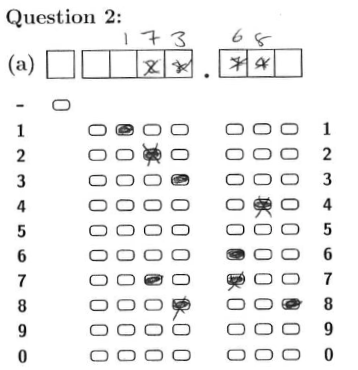
\includegraphics[width=8cm]{crossClash}\\
  \caption{Image showing answer with crossed out answers that the system misinterpreted.}
  \label{fig:crossClash}
\end{figure}

\subsubsection{Clashlist}

A total of 6 out of the 25 test where reported as clashes. The two images without a template were both reported in the clash list. Further the 1 test which only has the student number written in characters with no bubble information is also reported to the list. The other 3 clashes were reported due to the crossed out bubbles interpreted as still filled in, causing the system to think that two answer were filled in. An example of this can be seen in Figure \ref{fig:crossClash}.

\subsubsection{Incorrect automatic graded results}

There where 4 tests in total that where graded automatically, but incorrectly. All of these test were tests that had only character information in atleast one of the answers. An example of this can be seen in Figure \ref{fig:OnlyCharacters}

\begin{figure}
  \centering
  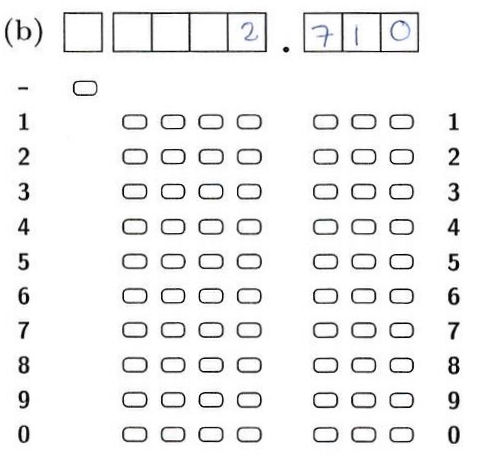
\includegraphics[width=8cm]{OnlyCharacters}\\
  \caption{Filled in answer with only character information.}
  \label{fig:OnlyCharacters}
\end{figure}

\subsection{Complete system}

\subsubsection{Marking statistics}

Using this complete system an average time for each test is calculated to be 2.011 seconds. 

\subsubsection{Clashlist}

A total of 6 out of the 25 test where reported as clashes. The two images with no template in were both again reported in the clash list. Two cases was reported to the clash list due to the character recognition determining a crossed out character as the intended character. An example of this is shown in Figure \ref{fig:crossedOutCharacter}. One test was reported due to it only having characters written in with no bubbles. Thus even though the system identified every character correctly, it had to low of a percentage faith in its answer and reported it to the clash list. 

\begin{figure}
  \centering
  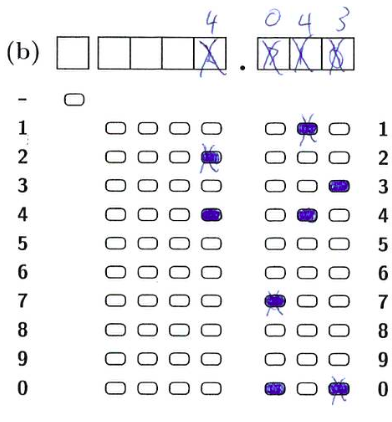
\includegraphics[width=8cm]{crossedOutCharacter}\\
  \caption{Crossed out character that confused the grading system.}
  \label{fig:crossedOutCharacter}
\end{figure}

\subsubsection{Incorrect automatic graded results}

There were no automatically graded answers that was done so incorrectly.

\subsection{Analysis or results}

As is seen in the section below, the complete systems does not reduce the number of clashes significantly for these 25 images. The complete system sometimes classifies a crossed out character as the intended character in that block. But because it is crossed out the system assigns a low certainty to that value, as the neural network is not to sure which digit it is. A drawback of the completed system is that it takes on average 2.011 seconds to grade a tests. This is due to the student number PGM taking on average 1.5 seconds to infer the correct student number. The complete system had no incorrectly automatically graded answers in contras to the 4 graded incorrectly using the basic system. A reason to this is attributed due to more evidence that gets considered in the complete system. Thus only if the evidence match up will the system be certain enough to accept its answer as the correct one. In the next section the complete system is used to grade a tutorial written by students. 

\section{Grading of tutorial tests}
In this section the complete system is tested on the final tutorial test written by the student class. Thus the final version of the complete system was used in grading the students' tests. To analyse the results student feedback is recorded to find tests that were graded incorrectly. 

\subsection{Marking statistics}

For these tutorial test  an average marking time per test of 2.3 seconds is recorded.

\subsection{Clashlist}

In total there were 67 clashes in the 888 tests. These 67 clashes are categorised in Table  \ref{tbl:TutClash}.
\begin{table}
  \centering
  \caption{Description and quantity of clashes in the different catagories.} \label{tbl:TutClash}
\begin{tabular}{|c|c|}
\hline
\textbf{Number of tests} & \textbf{Category description}\\
\textbf{in category} &\\
\hline
41&In these tests the system guessed the right values,\\ 
&but was unsure about its answer. Some of the\\
&cases was when the student number was only filled\\
&in the character box. The software always\\
&identified the correct student number, but was\\
&still unsure about that answer.\\
\hline
15&In these tests the system could not distinguish\\ 
&between a crossed out answer and correct answer.\\
&This is due to the crossed out answer being\\
&interpreted as a filled in answer.\\
\hline
8&These tests have an answer with only character\\ 
&information in them. The system tried to identify\\
&each answer, but made a mistake in atleast one of the\\
&digits.\\
\hline
2&These images contained blank papers that did not\\ 
&include test templates.\\
\hline
1&In this test the grid of the test paper can not be\\ 
&found. Thus the test could not be marked.\\
\hline
\end{tabular}
\end{table}

\subsection{Incorrect automatic graded results}

For this tutorial the students were asked to report any results that were marked incorrectly by the system. These results are all the results that the system decided to accept the automatically graded answer and in doing so graded the test incorrectly.

Only 1 result was reported where the software automatically marked the wrong answer to a test. The correct answer was -95.0 and the system marked the answer as 95.0, as seen in Figure \ref{fig:wrongAns}. There might still be test that were marked wrong, but these test(s) were not reported. In comparison there was 15 known mistakes made in in the first tutorial using the basic system.

\begin{figure}
  \centering
  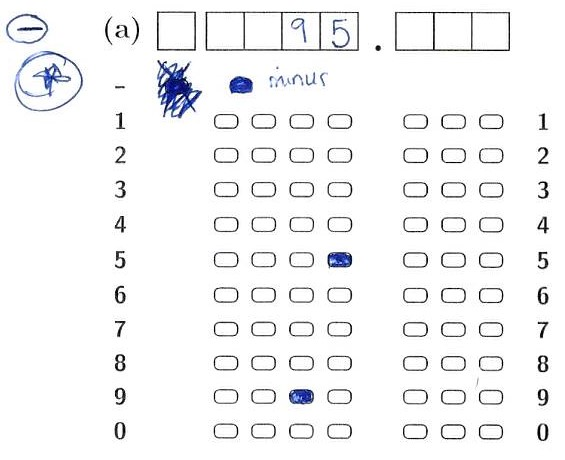
\includegraphics[width=8cm]{wrongResult}\\
  \caption{Incorrectly identified answer as 95.}
  \label{fig:wrongAns}
\end{figure}

For a more detailed description of the results from grading all 4 tutorial tests, refer to Appendix \ref{ap:results}.

\subsection{Analysis or results}

In conclusion it is noted that the complete system, with its machine learning capabilities, slightly reduces the number of tests that the user must mark manually from the previous basic system. About 7.5\% of the tests in the tutorial had to be marked manually, due to the system being unsure of its answers. The system does however have a high probability of grading tests correctly if they are done automatically. A reason for this can be attributed to the fact that the system correlates two pieces of evidence to predict the correct answer. Thus both the character and bubble information has to be interpreted incorrectly for the system to automatically grade a answer incorrectly. 

Thus overall the system could graded 92.5\% of all the test correctly and automatically. From the remaining 7.5\% only 1 test or 0.1\% of the tests was found to be graded wrongly. For the remaining 7.4\% of the tests the system was not certain enough to grade these test automatically. The system did classify most of the clashlist test correctly. This means the system could possible have graded 97.1\% of the tests correctly. This can be done by changing a threshold value, but allows the other 2.9\% of the tests to be classified incorrectly.

